\documentclass[UTF8]{ctexart}
\usepackage{amsmath}
\usepackage{mathtools}
\usepackage{geometry}
\usepackage{tikz}
\usepackage{enumitem}
\usepackage{ulem}
\setitemize{topsep=-0.3cm}
\geometry{a4paper,scale=0.75}
\title{每日一题(4.1)答案}
\author{选题:李衡岳,程昊一\\答案制作:程昊一}
\begin{document}
\maketitle
\begin{itemize}
\item[\textbf{1.}]{\CJKfamily{kai}用纯数学的方法证明圆锥的体积公式
\[V=\frac{1}{3}\pi r^2h\]
(李衡岳供题)}\\
\hspace*{2em}\textbf{解}\quad 我们在小学六年级时学到了圆锥的体积是等底等高的圆柱体积的$\frac{1}{3}$.可你有没有想过,系数“$\frac{1}{3}$”是如何产生的?\\
\hspace*{2em}我们通过具有“极限”思想的数学方法来证明圆锥的体积公式.首先,我们把圆锥沿平行于底面的方向将圆锥切成等高的$n$份.此时,每一份都是一个圆台,只有最上面的那一份是圆锥.我们记从上往下数的第$i$块为$S_i$,则对于$S_i$,它的下底面积为$\pi r^2\cdot (\dfrac{i}{n})^2$.我们把每一个圆台都近似地看成与这个圆台下底面相同、高相等的圆柱.注意:虽然我们进行的近似有误差,但是当$n$足够大时,这个误差会变得非常小,也就是说,当$n\to+\infty$时(“$\to$”表示“趋近于”),这个误差也将趋近于0.
\begin{figure}[!ht]
\centering
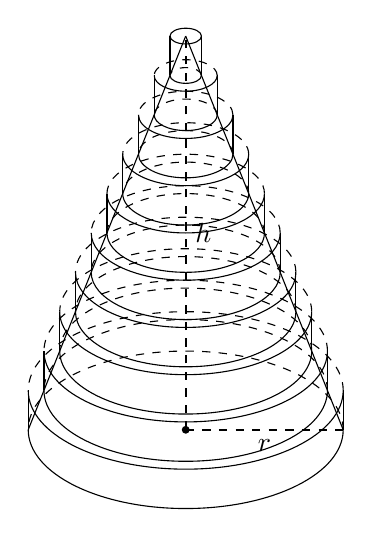
\begin{tikzpicture}
	\draw (0,5)--(2,0);
	\draw (0,5)--(-2,0);
	\fill (0,0) circle(0.05);
	\draw [thick,dashed](0,0)--(2,0);
	\draw [thick,dashed](0,0)--(0,5);
	\node at (1,0)[anchor=north]{$r$};
	\node at (0,2.5)[anchor=west]{$h$};

 	\draw (-2*0.1,5-5*0.1) arc(180:360:2*0.1 and 0.1);
	\draw [dashed](2*0.1,5-5*0.1) arc(0:180:2*0.1 and 0.1);
	\draw (2*0.1,5-5*0.1)--(2*0.1,5.5-5*0.1);
	\draw (-2*0.1,5-5*0.1)--(-2*0.1,5.5-5*0.1);
	\draw (-2*0.1,5.5-5*0.1) arc(180:360:2*0.1 and 0.1);
	\draw (2*0.1,5.5-5*0.1) arc(0:180:2*0.1 and 0.1);
	
	\draw (-2*0.2,5-5*0.2) arc(180:360:2*0.2 and 0.2);
	\draw [dashed](2*0.2,5-5*0.2) arc(0:180:2*0.2 and 0.2);
	\draw (2*0.2,5-5*0.2)--(2*0.2,5.5-5*0.2);
	\draw (-2*0.2,5-5*0.2)--(-2*0.2,5.5-5*0.2);
	\draw (-2*0.2,5.5-5*0.2) arc(180:360:2*0.2 and 0.2);
	\draw [dashed](2*0.2,5.5-5*0.2) arc(0:180:2*0.2 and 0.2);
	
 	\draw (-2*0.3,5-5*0.3) arc(180:360:2*0.3 and 0.3);
	\draw [dashed](2*0.3,5-5*0.3) arc(0:180:2*0.3 and 0.3);
	\draw (2*0.3,5-5*0.3)--(2*0.3,5.5-5*0.3);
	\draw (-2*0.3,5-5*0.3)--(-2*0.3,5.5-5*0.3);
	\draw (-2*0.3,5.5-5*0.3) arc(180:360:2*0.3 and 0.3);
	\draw [dashed](2*0.3,5.5-5*0.3) arc(0:180:2*0.3 and 0.3);
	
 	\draw (-2*0.4,5-5*0.4) arc(180:360:2*0.4 and 0.4);
	\draw [dashed](2*0.4,5-5*0.4) arc(0:180:2*0.4 and 0.4);
	\draw (2*0.4,5-5*0.4)--(2*0.4,5.5-5*0.4);
	\draw (-2*0.4,5-5*0.4)--(-2*0.4,5.5-5*0.4);
	\draw (-2*0.4,5.5-5*0.4) arc(180:360:2*0.4 and 0.4);
	\draw [dashed](2*0.4,5.5-5*0.4) arc(0:180:2*0.4 and 0.4);
	
 	\draw (-2*0.5,5-5*0.5) arc(180:360:2*0.5 and 0.5);
	\draw [dashed](2*0.5,5-5*0.5) arc(0:180:2*0.5 and 0.5);
	\draw (2*0.5,5-5*0.5)--(2*0.5,5.5-5*0.5);
	\draw (-2*0.5,5-5*0.5)--(-2*0.5,5.5-5*0.5);
	\draw (-2*0.5,5.5-5*0.5) arc(180:360:2*0.5 and 0.5);
	\draw [dashed](2*0.5,5.5-5*0.5) arc(0:180:2*0.5 and 0.5);
	
 	\draw (-2*0.6,5-5*0.6) arc(180:360:2*0.6 and 0.6);
	\draw [dashed](2*0.6,5-5*0.6) arc(0:180:2*0.6 and 0.6);
	\draw (2*0.6,5-5*0.6)--(2*0.6,5.5-5*0.6);
	\draw (-2*0.6,5-5*0.6)--(-2*0.6,5.5-5*0.6);
	\draw (-2*0.6,5.5-5*0.6) arc(180:360:2*0.6 and 0.6);
	\draw [dashed](2*0.6,5.5-5*0.6) arc(0:180:2*0.6 and 0.6);
	
 	\draw (-2*0.7,5-5*0.7) arc(180:360:2*0.7 and 0.7);
	\draw [dashed](2*0.7,5-5*0.7) arc(0:180:2*0.7 and 0.7);
	\draw (2*0.7,5-5*0.7)--(2*0.7,5.5-5*0.7);
	\draw (-2*0.7,5-5*0.7)--(-2*0.7,5.5-5*0.7);
	\draw (-2*0.7,5.5-5*0.7) arc(180:360:2*0.7 and 0.7);
	\draw [dashed](2*0.7,5.5-5*0.7) arc(0:180:2*0.7 and 0.7);
	
 	\draw (-2*0.8,5-5*0.8) arc(180:360:2*0.8 and 0.8);
	\draw [dashed](2*0.8,5-5*0.8) arc(0:180:2*0.8 and 0.8);
	\draw (2*0.8,5-5*0.8)--(2*0.8,5.5-5*0.8);
	\draw (-2*0.8,5-5*0.8)--(-2*0.8,5.5-5*0.8);
	\draw (-2*0.8,5.5-5*0.8) arc(180:360:2*0.8 and 0.8);
	\draw [dashed](2*0.8,5.5-5*0.8) arc(0:180:2*0.8 and 0.8);
	
 	\draw (-2*0.9,5-5*0.9) arc(180:360:2*0.9 and 0.9);
	\draw [dashed](2*0.9,5-5*0.9) arc(0:180:2*0.9 and 0.9);
	\draw (2*0.9,5-5*0.9)--(2*0.9,5.5-5*0.9);
	\draw (-2*0.9,5-5*0.9)--(-2*0.9,5.5-5*0.9);
	\draw (-2*0.9,5.5-5*0.9) arc(180:360:2*0.9 and 0.9);
	\draw [dashed](2*0.9,5.5-5*0.9) arc(0:180:2*0.9 and 0.9);
	
 	\draw (-2*1,5-5*1) arc(180:360:2*1 and 1);
	\draw [dashed](2*1,5-5*1) arc(0:180:2*1 and 1);
	\draw (2*1,5-5*1)--(2*1,5.5-5*1);
	\draw (-2*1,5-5*1)--(-2*1,5.5-5*1);
	\draw (-2*1,5.5-5*1) arc(180:360:2*1 and 1);
	\draw [dashed](2*1,5.5-5*1) arc(0:180:2*1 and 1);
	
\end{tikzpicture}
\end{figure}

\hspace*{2em}对于每一个圆柱,我们记从上往下数的第$i$个圆柱(也就是$S_i$对应的圆台)的体积为$V_i$.则我们有
\[\frac{h}{n}\cdot \pi r^2\cdot (\dfrac{i}{n})^2\]
即
\[\frac{\pi r^2 h}{n^3}\cdot i^2\]
\hspace*{2em}所以,圆锥的体积$V$
\begin{align*}
&=\sum\limits_{i=1}^{n} V_i\\
&=\sum\limits_{i=1}^{n} \frac{\pi r^2h}{n^3}\cdot i^2\\
&=\frac{\pi r^2h}{n^3} \sum\limits_{i=1}^{n}i^2\\
&=\frac{\pi r^2h}{n^3}\cdot \frac{n(n+1)(2n+1)}{6}\\
&=\pi r^2h\cdot \frac{(n+1)(2n+1)}{6n^2}\\
\end{align*}
\hspace*{2em}其中$\sum$的用法参见\uline{https://baike.baidu.com/item/∑/1233796}.\\
\hspace*{2em}现在,我们来看$\dfrac{(n+1)(2n+1)}{6n^2}$在$n\to+\infty$时的值.我们对这个式子做一个变形:
\begin{align*}
&\frac{(n+1)(2n+1)}{6n^2}\\
=&\frac{\frac{n+1}{n}\cdot\frac{2n+1}{n}}{\frac{6n^2}{n^2}}\quad\text{(分子分母同时除以$n^2$)}\\
=&\frac{(1+\frac{1}{n})(2+\frac{1}{n})}{6}\quad\text{(整理式子)}\\
\end{align*}
我们知道,当$n\to \infty$时,$\frac{1}{n}\to 0$.所以,当$n\to\infty$时,$\dfrac{(1+\frac{1}{n})(2+\frac{1}{n})}{6}\to\dfrac{(1+0)(2+0)}{6}=\dfrac{1}{3}$.\\
\hspace*{2em}所以,在$n\to+\infty$时,
\[V=\pi r^2h\cdot \frac{(n+1)(2n+1)}{6n^2}\to\frac{1}{3}\pi r^2h\]
\hspace*{2em}至此,我们证明了圆锥的体积公式.\\
\hspace*{2em}\textbf{注}\quad 这道题最严格的表述如下(有兴趣的同学可以看一下):
\begin{align*}
V&=\int_0^h \pi(r\cdot\frac{x}{h})^2{\rm d}x\\
&=\frac{\pi r^2}{h^2}\int_0^h x^2{\rm d}x\\
&=\frac{\pi r^2}{h^2}\cdot\left(\left.\frac{1}{3}x^3\right|_0^h\right)\\
&=\frac{\pi r^2}{h^2}\cdot \frac{1}{3}h^3\\
&=\frac{1}{3}\pi r^2h
\end{align*}
\item[\textbf{2.}]{\CJKfamily{kai}求所有的整数$x,y$,使得$x^2+xy+y^2=1$.\\
(程昊一供题)}\\
\hspace*{2em}\textbf{分析}\quad 看到这个式子,我们能很容易地发现$x,y$都为正整数时不成立,因为$x^2+xy+y^2\ge 1^2+1\times 1+1^2>1$.注意:我们在这里是利用\textbf{不等关系}导出的矛盾,所以说,这提示我们将要利用不等关系解决此题.更一般地,解决不定方程的基本方法就是:因式分解、同余、不等关系等.\\
\hspace*{2em}\textbf{解}\quad 若$xy>0$即$xy\ge1$,则$x\neq0,y\neq 0$,所以$x^2+xy+y^2\ge 1+1+1>1$,矛盾.\\
\hspace*{2em}若$xy=0$,则通过枚举我们可以得到$(x,y)=(0,\pm1)或(\pm1,0)$.\\
\hspace*{2em}若$xy<0$,即$xy\le-1$,我们将原方程做变形:
\[x^2+xy+y^2=1\Leftrightarrow x^2+2xy+y^2=1+xy\Leftrightarrow (x+y)^2=1+xy\]
由于平方的非负性,我们得到$1+xy\ge0$,即$xy\ge-1$,又$xy\le-1$,所以$xy=-1$.\\
于是枚举立得$(x,y)=(\pm1,\mp1)$.\\
\hspace*{2em}综上:原方程的解为$(x,y)=(0,\pm1)$或$(\pm1,0)$或$(\pm1,\mp1)$.


\end{itemize}
\end{document}